% Complete Section 4.3, original PDF 47-49 / printed 37-39.
% block: l2-de-rham-heading page:47 type:section
\subsection{\BT{Example: The $L^2$ de Rham complex}{Example: $L^2$ de Rham 复形}}\label{sec:l2-de-rham-complex}

% block: l2-de-rham-base-domain page:47 type:ordinary-paragraph
\BT{The prototypical example of a Hilbert complex is the de Rham complex associated to a Riemannian manifold. We continue to discuss the case of a domain $\Omega$ in $\mathbb R^3$, which we shall assume to have a Lipschitz boundary. The base Hilbert spaces will be $W^0=W^3=L^2(\Omega)$, $W^1=W^2=L^2(\Omega;\mathbb R^3)$. The operators are the ones discussed in Section~\ref{sec:vector-operators-adjoints}: $d^0=\operatorname{grad}$, $d^1=\operatorname{curl}$, $d^2=\operatorname{div}$, with the domains taken to be $H^1$, $H(\operatorname{curl})$, and $H(\operatorname{div})$, respectively. We saw there that these are closed operators, so we meet the criteria for a Hilbert complex. The domain complex, consisting of the spaces $V^k$, is}{Hilbert 复形的典型例子是与 Riemannian 流形相伴的 de Rham 复形. 继续讨论 $\mathbb R^3$ 中区域 $\Omega$ 的情形, 并假设其具有 Lipschitz 边界. 基 Hilbert 空间取为 $W^0=W^3=L^2(\Omega)$, $W^1=W^2=L^2(\Omega;\mathbb R^3)$. 算子是 Section~\ref{sec:vector-operators-adjoints} 中讨论的那些算子: $d^0=\operatorname{grad}$, $d^1=\operatorname{curl}$, $d^2=\operatorname{div}$, 定义域分别取为 $H^1$, $H(\operatorname{curl})$ 和 $H(\operatorname{div})$. 那里已看到这些算子是闭的, 因而满足 Hilbert 复形的条件. 由空间 $V^k$ 组成的定义域复形为}
\begin{equation}\label{eq:l2-de-rham-domain-complex}
0\to H^1\xrightarrow{\operatorname{grad}}H(\operatorname{curl})\xrightarrow{\operatorname{curl}}H(\operatorname{div})\xrightarrow{\operatorname{div}}L^2\to0.
\end{equation}

% block: l2-dual-domain-complex page:47 type:ordinary-paragraph
\BT{In view of the adjoints computed in Section~\ref{sec:vector-operators-adjoints}, the domain complex of the dual complex (consisting of the $V_k^*$) is}{根据 Section~\ref{sec:vector-operators-adjoints} 中计算的伴随, 对偶复形的定义域复形 (由 $V_k^*$ 组成) 为}
\begin{equation}\label{eq:l2-dual-domain-complex}
0\leftarrow L^2\xleftarrow{-\operatorname{div}}\mathring H(\operatorname{div})\xleftarrow{\operatorname{curl}}\mathring H(\operatorname{curl})\xleftarrow{-\operatorname{grad}}\mathring H^1\leftarrow0.
\end{equation}

% block: de-rham-compactness page:48 type:ordinary-paragraph
\BT{An important fact is that the $L^2$ de Rham complex satisfies the compactness property, i.e., that $V^k\cap V_k^*$ is compactly included in $W^k$. For $k=0$, we have $V^0\cap V_0^*=H^1\cap L^2=H^1$ which is indeed compact in $W^0=L^2$ by Rellich's theorem. The result for $k=3$ is similar. For $k=1$ and $2$ the desired results are that $H(\operatorname{curl})\cap\mathring H(\operatorname{div})$ and $\mathring H(\operatorname{curl})\cap H(\operatorname{div})$ are compact in $L^2(\Omega;\mathbb R^3)$. This was proved, in the greater generality of Riemannian manifolds with Lipschitz boundary, by Picard \BookCite{62}. According to Theorem~\ref{thm:compactness-implies-fredholm}, the compactness property implies that the de Rham complex is Fredholm: the operators have closed range, and the harmonic form spaces are finite dimensional. In particular, we have established that $\operatorname{curl}H(\operatorname{curl})$ is closed, as claimed at the end of Chapter~\ref{chap:unbounded-operators}. We now calculate the spaces of harmonic forms and exhibit the Hodge decomposition for each degree.}{一个重要事实是, $L^2$ de Rham 复形满足紧性性质, 即 $V^k\cap V_k^*$ 紧嵌入 $W^k$. 对 $k=0$, 有 $V^0\cap V_0^*=H^1\cap L^2=H^1$, 由 Rellich 定理, 它在 $W^0=L^2$ 中确实是紧的. $k=3$ 的结论类似. 对 $k=1$ 和 $2$, 所需结论是 $H(\operatorname{curl})\cap\mathring H(\operatorname{div})$ 与 $\mathring H(\operatorname{curl})\cap H(\operatorname{div})$ 在 $L^2(\Omega;\mathbb R^3)$ 中紧. Picard \BookCite{62} 在具有 Lipschitz 边界的 Riemannian 流形这一更一般背景下证明了此结论. 根据 Theorem~\ref{thm:compactness-implies-fredholm}, 紧性性质意味着 de Rham 复形是 Fredholm 的: 各算子的像空间是闭的, 且调和形式空间为有限维. 特别地, 我们已证明 $\operatorname{curl}H(\operatorname{curl})$ 是闭的, 正如 Chapter~\ref{chap:unbounded-operators} 末尾所述. 下面计算调和形式空间, 并给出每个次数上的 Hodge 分解.}

% block: harmonic-zero-forms page:48 type:ordinary-paragraph
\BT{The space of harmonic $0$-forms coincides with $\mathcal Z^0$, the null space of the gradient. This is the space of constants, or, if we allow domains with more than the one connected component, the space of local constants. Its dimension is the number $b_0$ of connected components of $\Omega$ (the zeroth Betti number of the domain). Since the space $\mathcal B^0=0$, the Hodge decomposition expresses $L^2$ as the sum $\operatorname{div}\mathring H(\operatorname{div})$ and the constant (or locally constant) functions.}{调和 $0$-形式的空间与梯度的零空间 $\mathcal Z^0$ 相同. 这是常数空间, 或者若允许区域有多个连通分支, 则是局部常数空间. 其维数是 $\Omega$ 的连通分支数 $b_0$ (即区域的第零个 Betti 数). 由于空间 $\mathcal B^0=0$, Hodge 分解将 $L^2$ 表示为 $\operatorname{div}\mathring H(\operatorname{div})$ 与常数 (或局部常数) 函数之和.}

% block: harmonic-one-forms pages:48,49 type:ordinary-paragraph
\BT{The space of harmonic $1$-forms is more complicated. It consists of the $L^2$ vector fields $p$ for which $\operatorname{curl}p=0$, $\operatorname{div}p=0$, and the normal trace $\gamma_n p$ vanishes on $\partial\Omega$. An elementary example of such a function is pictured on the left of Figure~\ref{fig:de-rham-harmonic-fields}, in which the domain is an annular cylinder. In cylindrical coordinates the domain is given by $a\leq r\leq b$, $c\leq z\leq d$, for some $0<a<b$, $c<d$, and the harmonic forms are simply the multiples of $p=\operatorname{grad}\theta$. On a general domain $\dim\mathsf H^1=b_1$, the first Betti number, which we defined in Section~\ref{sec:simplicial-chain-complex} and which counts the number of tunnels through the domain. For a simply connected domain, $b_1=0$, and the Hodge decomposition is the classical Helmholtz decomposition of a vector field into a gradient (which is irrotational, meaning curl-free) and a curl (solenoidal, meaning divergence-free). For a general domain, we must also include the harmonic part:}{调和 $1$-形式的空间更复杂. 它由满足 $\operatorname{curl}p=0$, $\operatorname{div}p=0$, 且法向迹 $\gamma_n p$ 在 $\partial\Omega$ 上为零的 $L^2$ 向量场 $p$ 组成. Figure~\ref{fig:de-rham-harmonic-fields} 左图给出了这种函数的一个初等例子, 其区域是环形柱体. 在柱坐标中, 该区域由 $a\leq r\leq b$, $c\leq z\leq d$ 给出, 其中 $0<a<b$, $c<d$, 而调和形式就是 $p=\operatorname{grad}\theta$ 的倍数. 在一般区域上, $\dim\mathsf H^1=b_1$, 即第一个 Betti 数, 它在 Section~\ref{sec:simplicial-chain-complex} 中已定义, 计数贯通区域的隧道数. 对单连通区域, $b_1=0$, Hodge 分解就是经典的 Helmholtz 分解, 将向量场分解为一个梯度 (无旋的, 即旋度为零) 和一个旋度 (螺线的, 即散度为零). 对一般区域, 还必须包含调和部分:}
\[
L^2(\Omega;\mathbb R^3)=\operatorname{grad}H^1(\Omega)\BookOrthSum\operatorname{curl}\mathring H(\operatorname{curl};\Omega)\BookOrthSum\mathsf H^1.
\]

% block: de-rham-harmonic-fields-figure page:48 type:figure
\begin{figure}[htbp]\centering
\includegraphics[page=48,trim=89bp 83bp 57bp 445bp,clip,width=.85\linewidth]{../input/source/Finite Element Exterior Calculus.pdf}
\caption{\BT{Left: Harmonic $1$-form on an annular cylinder in $\mathbb R^3$. Right: Harmonic $2$-form on a spherical shell (half the shell has been cut away for visibility).}{左: $\mathbb R^3$ 中环形柱体上的调和 $1$-形式. 右: 球壳上的调和 $2$-形式 (为便于观察, 已切去半个球壳).}}\label{fig:de-rham-harmonic-fields}
\end{figure}

% block: harmonic-two-forms page:49 type:ordinary-paragraph
\BT{The space of harmonic $2$-forms consists of vector fields which are again curl- and divergence-free but, in this case, with vanishing tangential trace on the boundary. An elementary example is given in spherical coordinates on the closed spherical shell $a<r<b$ by $p=\operatorname{grad}(1/r)$. See Figure~\ref{fig:de-rham-harmonic-fields}. On a general domain, $\dim\mathsf H^2=b_2$, the number of voids in the domain. The Hodge decomposition is again into gradients and curls, but the boundary conditions are different, as is the space of harmonic forms:}{调和 $2$-形式的空间同样由无旋且无散的向量场组成, 但此时它们在边界上的切向迹为零. 一个初等例子是在闭球壳 $a<r<b$ 上, 用球坐标给出的 $p=\operatorname{grad}(1/r)$. 见 Figure~\ref{fig:de-rham-harmonic-fields}. 在一般区域上, $\dim\mathsf H^2=b_2$, 即区域中的空腔数. Hodge 分解仍然分解为梯度和旋度, 但边界条件不同, 调和形式空间也不同:}
\[
L^2(\Omega;\mathbb R^3)=\operatorname{grad}\mathring H^1(\Omega)\BookOrthSum\operatorname{curl}H(\operatorname{curl};\Omega)\BookOrthSum\mathsf H^2.
\]

% block: harmonic-three-forms page:49 type:ordinary-paragraph
\BT{Finally, the space of harmonic $3$-forms is simple: $\mathsf H^3=0$, since there are no nonzero functions in $\mathring H^1$ with vanishing gradient. Of course, $\mathcal B_3^*$ also vanishes, so the Hodge decomposition is trivial.}{最后, 调和 $3$-形式的空间很简单: $\mathsf H^3=0$, 因为 $\mathring H^1$ 中没有梯度为零的非零函数. 当然, $\mathcal B_3^*$ 也为零, 因此 Hodge 分解是平凡的.}
